% begin module algebraic-functions
\begin{frame}
\frametitle{Algebraic Functions}
\begin{definition}[Algebraic Function]
An algebraic function is a function that can be constructed using algebraic operations (such as addition, subtraction, multiplication, division, and taking roots) starting from polynomials.
\end{definition}
\uncover<2->{
Algebraic functions can look pretty funny.
\begin{tabular}{ccc}
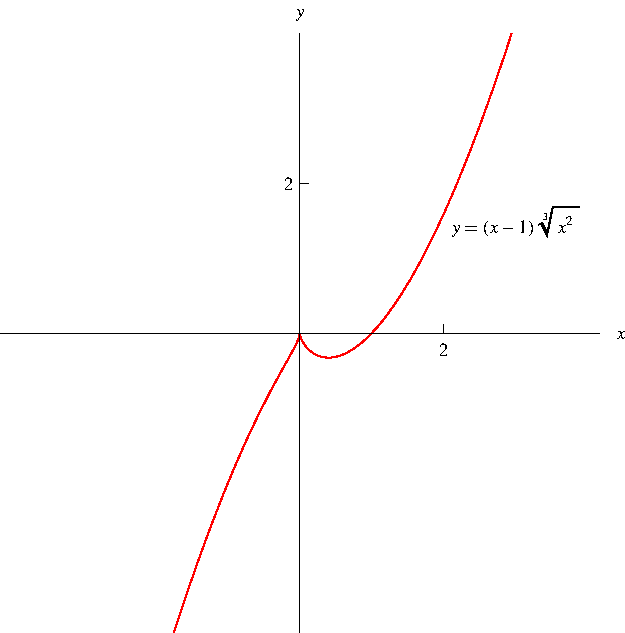
\includegraphics[height=3.8cm]{precalculus/pictures/01-02-algebraic1.pdf}&%
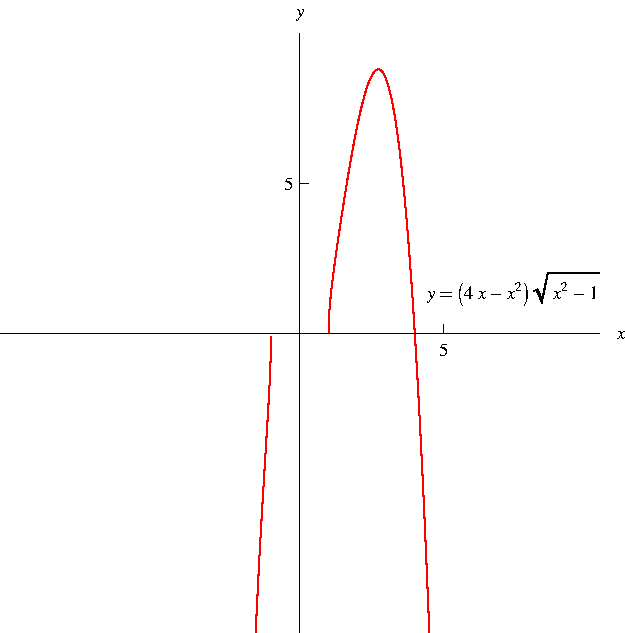
\includegraphics[height=3.8cm]{precalculus/pictures/01-02-algebraic2.pdf}&%
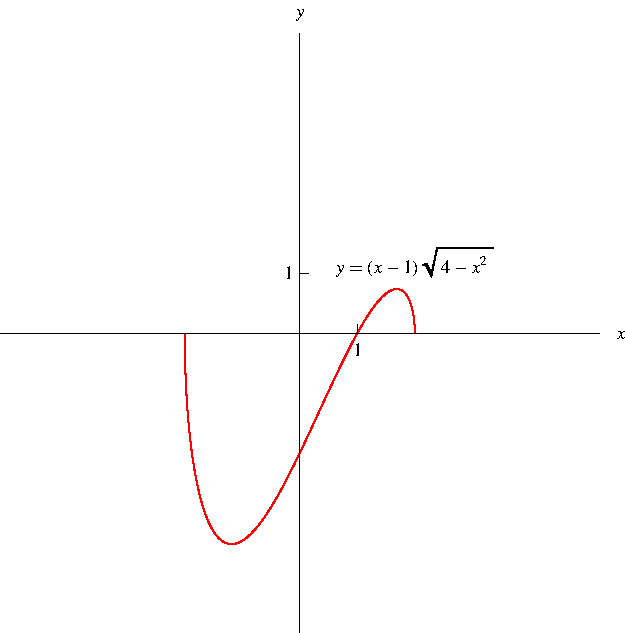
\includegraphics[height=3.8cm]{precalculus/pictures/01-02-algebraic3.pdf}%
\end{tabular}
}
\end{frame}
% end module algebraic-functions
